\documentclass[conference,a4paper]{IEEEtran}
\usepackage[utf8]{inputenc}
\usepackage[T1]{fontenc}
\usepackage{babel}
\babelprovide[main,import]{portuguese}
\usepackage{lmodern,microtype,booktabs,array,tikz,pgfplots}
\usepackage[hidelinks]{hyperref}
\usetikzlibrary{arrows.meta,positioning,babel}
\pgfplotsset{compat=1.18}
\newcommand{\code}[1]{\texttt{\small #1}}
\title{Deteção, monitorização e prevenção de ameaças numa arquitetura de serviços com vários sites}
\author{\IEEEauthorblockN{Guilherme Tavares (119867)}
\IEEEauthorblockA{Mestrado em Cibersegurança --- Segurança em Sistemas de Larga Escala\\
Universidade de Aveiro\\Projeto 1, novembro de 2026}}
\begin{document}
\maketitle

\begin{abstract}
Apresenta-se um sistema de telemetria de temperaturas com dois sites, Lisboa e Porto, no mesmo cluster K3s, executado numa VM Kali com Incus. Um gateway nginx partilhado recebe as consultas, a ingestão aceita leituras por HTTPS com token ou certificado de cliente, o Prometheus global federa agregados por site e o Wazuh recebe registos e alertas. Tratam-se três ameaças dos guiões práticos: negação de serviço por uma origem e por uma botnet, spam com fraude e exploração do gateway com Shellshock. A publicação não autorizada de leituras e a interceção da publicação ficam como extras. Uma reputação partilhada bloqueia em todos os serviços a origem que reincide. Todos os ensaios usam tráfego real de contentores de ataque e foram repetidos cinco vezes. Com a mesma carga, o p95 do cliente legítimo passou de 681~ms sem proteção para 2,9~ms com proteção. Na mediana das repetições, o atacante ficou bloqueado aos 1,6~s na rajada, aos 6~s no ataque de três bots, aos 2,3~s no spam e aos 1,3~s no Shellshock, sem nenhum erro do cliente legítimo. Nenhuma mensagem de spam chegou à caixa e, no extra da publicação, nenhuma leitura forjada foi gravada.
\end{abstract}

\begin{IEEEkeywords}
SOA, K3s, Prometheus, Wazuh, DDoS, botnet, spam, autorização, correlação.
\end{IEEEkeywords}

\section{Introdução}
O Projeto~1 pede uma arquitetura de serviços capaz de crescer, identificação dos elementos por localização, monitorização com Prometheus e o tratamento de três ameaças do programa com deteção e resposta no SIEM~\cite{course}. A aplicação recolhe temperaturas. Sensores publicam leituras e clientes consultam a média ou a lista de leituras de cada site.

Os três cenários principais seguem temas tratados nos guiões práticos. São a negação de serviço, também na variante distribuída por uma botnet, o correio não solicitado com mensagens de fraude e a exploração de um serviço exposto com o Shellshock. Em cada um, o projeto parte da montagem do guião e acrescenta o que ela não tinha, como resposta automática medida, quarentena, correlação ou reputação. Ficam como extras a publicação de leituras sem credencial, uma forma de sequestro de sinais, e a interceção da ligação do sensor. Para cada cenário, o artigo descreve a ameaça, a forma de exploração, os sinais monitorizados, a resposta e o resultado medido. O critério de sucesso é o efeito sobre o atacante e sobre o utilizador legítimo, além do alerta que chega ao operador. O código, a configuração, as evidências dos ensaios e os vídeos das demonstrações, um por ataque na pasta \code{demo/}, estão em \url{https://github.com/T4V4RES/SSLE-P1}.

\section{Estado da arte}
Uma arquitetura orientada a serviços separa responsabilidades e permite replicar as etapas com maior procura. Em Kubernetes, os Services dão aos consumidores um nome estável mesmo quando mudam os pods, e as políticas de rede restringem as ligações entre componentes~\cite{knet}. A federação Prometheus separa a recolha local da observação global e deixa o detalhe perto do serviço que o produz~\cite{prom}.

O SIEM normaliza registos de várias fontes e aplica regras que relacionam sinais de um incidente~\cite{bhatt,wazuh}. No Wazuh, a resposta ativa envia uma ação ao agente que a executa, por exemplo uma regra na firewall local contra a origem identificada~\cite{wazuhar}. A correlação entre sintomas de desempenho e eventos de segurança ajuda a passar da deteção ao diagnóstico, como prevê o ciclo de gestão de falhas~\cite{m3400}.

Na negação de serviço por volume, filtrar perto da entrada poupa trabalho ao sistema que recebe a carga. A quantidade de pedidos também é compatível com uma afluência legítima concentrada, o que obriga a separar o volume da origem~\cite{mirkovic,jung}. No nginx, o limite de pedidos usa um balde com margem de rajada por chave, e o limite de ligações conta as ligações em curso~\cite{nginx}. No correio, o SpamAssassin soma regras de conteúdo e de cabeçalhos numa pontuação. Para isso precisa de saber que relés são de confiança~\cite{sa}. Na ingestão, o TLS protege o transporte e a autorização associa a credencial ao identificador do sensor.

\section{Arquitetura de serviços}
A VM Kali aloja seis contentores Incus de serviço. \code{k3s-master} e \code{k3s-node1} são os dois nós de um único cluster. O nginx corre em \code{ssle-gateway} e o Postfix, o SpamAssassin e o Dovecot em \code{lis-mail}. O \code{prom-global} aloja o Prometheus global, o Alertmanager e o recetor de webhooks, e o \code{wazuh-container} o gestor do SIEM. Os clientes de ensaio \code{bot-1}, \code{bot-2}, \code{bot-3} e \code{client-user} ficam parados e só arrancam durante os ensaios. A Fig.~\ref{fig:arquitetura} resume a instalação.

\begin{figure*}[!t]
\centering
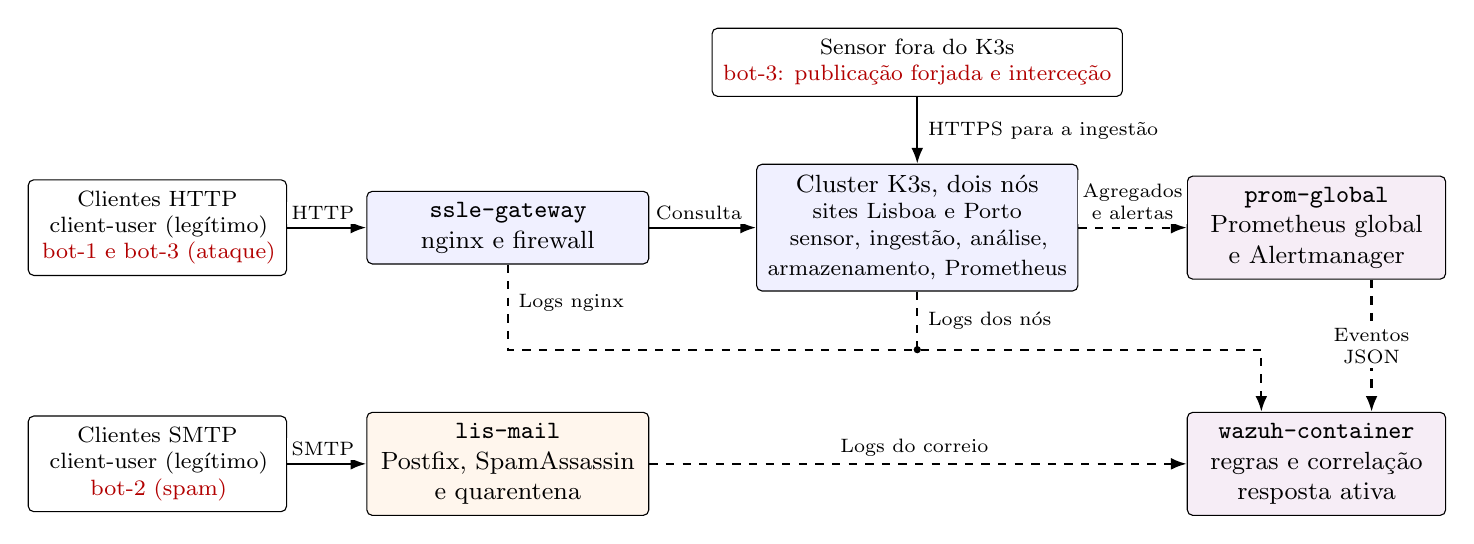
\begin{tikzpicture}[
  box/.style={draw, rounded corners=2pt, align=center, font=\small, inner sep=4pt},
  client/.style={box, font=\footnotesize, text width=3.0cm},
  svc/.style={box, text width=3.3cm},
  route/.style={-{Latex[length=2mm]}, thick},
  observ/.style={route, dashed},
  lab/.style={font=\scriptsize, inner sep=1.5pt, fill=white, align=center}
]
% Colunas: clientes, entrada, sites, observação. Linhas: HTTP (y=1.6) e SMTP (y=-1.4).
\node[client] (api) at (0,1.6) {Clientes HTTP\\client-user (legítimo)\\\textcolor{red!70!black}{bot-1 e bot-3 (ataque)}};
\node[client] (mailc) at (0,-1.4) {Clientes SMTP\\client-user (legítimo)\\\textcolor{red!70!black}{bot-2 (spam)}};
\node[svc, fill=blue!6] (ng) at (4.45,1.6) {\code{ssle-gateway}\\nginx e firewall};
\node[svc, fill=orange!7] (mail) at (4.45,-1.4) {\code{lis-mail}\\Postfix, SpamAssassin\\e quarentena};
\node[box, fill=blue!6, text width=3.8cm] (k3s) at (9.65,1.6)
 {Cluster K3s, dois nós\\{\footnotesize sites Lisboa e Porto\\sensor, ingestão, análise,\\armazenamento, Prometheus}};
\node[box, font=\footnotesize] (sens) at (9.65,3.7) {Sensor fora do K3s\\\textcolor{red!70!black}{bot-3: publicação forjada e interceção}};
\node[svc, fill=violet!7, text width=3.0cm] (pg) at (14.72,1.6) {\code{prom-global}\\Prometheus global\\e Alertmanager};
\node[svc, fill=violet!7, text width=3.0cm] (w) at (14.72,-1.4) {\code{wazuh-container}\\regras e correlação\\resposta ativa};
% Pedidos
\draw[route] (api) -- node[lab, above=1pt] {HTTP} (ng);
\draw[route] (mailc) -- node[lab, above=1pt] {SMTP} (mail);
\draw[route] (ng) -- node[lab, above=1pt] {Consulta} (k3s);
\draw[route] (sens) -- node[lab, right=2pt] {HTTPS para a ingestão} (k3s);
% Observação
\coordinate (bus) at (0,0.05);
\coordinate (wl) at ([xshift=-7mm]w.north);
\coordinate (wr) at ([xshift=7mm]w.north);
\draw[observ] (k3s) -- node[lab, above=1pt] {Agregados\\e alertas} (pg);
\draw[observ] (pg.south -| wr) -- node[lab] {Eventos\\JSON} (wr);
\draw[observ] (ng.south) -- node[lab, right=2pt, pos=0.45] {Logs nginx} (ng.south |- bus) -- (wl |- bus) -- (wl);
\draw[dashed, thick] (k3s.south) -- node[lab, right=2pt] {Logs dos nós} (k3s.south |- bus);
\fill (k3s.south |- bus) circle (1.3pt);
\draw[observ] (mail) -- node[lab, above=1pt] {Logs do correio} (w);
\end{tikzpicture}
\caption{Instalação na VM Kali. Cada caixa colorida é um contentor Incus; o K3s ocupa dois. As setas tracejadas mostram fluxos de observação e a vermelho estão as origens de ataque usadas nos ensaios. Os agentes Wazuh do gateway, do correio e dos dois nós K3s executam a resposta ativa do gestor na firewall local.}
\label{fig:arquitetura}
\end{figure*}

\subsection{Percursos de leitura e de escrita}
Cada namespace tem um sensor, duas réplicas de ingestão, duas de análise, um serviço de armazenamento com SQLite num volume persistente local e um Prometheus. No plano de leitura, o nginx recebe consultas de Lisboa na porta~80 e do Porto na~8080 e encaminha-as para o Service de análise do site pelos NodePorts~30501 e~30502. A política de rede só aceita nesses pods ligações do IP do gateway, pelo que um cliente não contorna o nginx. A análise pede a lista ao serviço \code{storage}, que executa a consulta SQL.

Um sensor dentro do namespace publica diretamente no Service HTTPS de ingestão. Para sensores fora do K3s, as portas são~30441 e~30442. A ingestão valida o identificador, a leitura e a credencial antes de contactar o armazenamento. Só uma escrita confirmada devolve \code{202}.

\subsection{Identificação e monitorização}
O Prometheus de cada site descobre os pods pela API do Kubernetes. As etiquetas de site, serviço, nó, bastidor e instância localizam um alerta. O identificador de cada elemento segue a forma \code{pt.<site>.dc1.rack1.<nó>.<função>.<instância>}. O namespace dá âmbito aos nomes dos Services e aos dados.

Cada Prometheus local guarda as séries por réplica e calcula agregados com prefixo \code{site:}. O global federa só esses agregados e recolhe as métricas do nginx. O Prometheus de cada site só aceita ligações do global: o Service preserva o IP de origem e a política de rede só admite esse endereço. Os alertas dos dois níveis seguem para o Alertmanager em \code{prom-global}. Um webhook converte-os em eventos JSON que o agente local envia ao Wazuh. Os agentes do gateway, do correio e dos dois nós K3s enviam os seus registos ao mesmo gestor. Um correlacionador no gestor lê os alertas e emite um evento quando um ataque e um sintoma de desempenho coincidem no mesmo site em 120~s. O mesmo processo guarda o historial de bloqueios de cada origem.

\subsection{Escolha do gateway}
Nos guiões das aulas, o Apache era o servidor-vítima: recebia a carga do ApacheBench no guião de DoS e o pedido Shellshock no guião do Wazuh. Neste projeto, o servidor web tem outra função. É o ponto de entrada partilhado à frente dos serviços dos dois sites, e é aí que se aplica o controlo de admissão. O nginx tem no núcleo o limite de pedidos por chave com margem de rajada e o limite de ligações por chave~\cite{nginx}. No Apache, o \code{mod\_ratelimit} do núcleo limita a largura de banda de cada resposta e não a taxa de pedidos. Uma limitação por cliente exigiria módulos externos como o \code{mod\_evasive}. O modelo orientado a eventos do nginx também evita reservar um processo ou uma thread por ligação, que é o recurso que os ataques de ligações lentas esgotam nos MPM \code{prefork} e \code{worker} do Apache~\cite{apachempm}. Os registos de acesso usam o mesmo formato combinado, por isso o descodificador e as regras web do Wazuh usados nas aulas funcionam sem alterações.

O gateway fica num contentor Incus e não num Ingress dentro do K3s. Assim, o agente Wazuh lê os logs e a resposta ativa altera a firewall sem dar privilégios a um pod. Os pods dos sites correm com a política \emph{restricted} do Kubernetes. Os nomes \code{.incus} dos contentores principais, usados pelo nginx, pela federação e pelo Alertmanager, estão fixos no dnsmasq da bridge (\code{host-record}) e não dependem das concessões DHCP. O \code{infra/check-after-boot.sh} confirma a resolução, a configuração do nginx, os alvos do Prometheus, os alertas ativos e os agentes antes de cada demonstração.


\section{Gestão de risco e mitigação}
A superfície de entrada tem quatro interfaces (Tabela~\ref{tab:defesas}), cada uma com um controlo próprio. A reincidência liga-as: a origem que volta a ser bloqueada, em qualquer serviço, perde o acesso a todos. A API de leitura é sensível a pedidos excessivos, e o gateway que a serve recebe também pedidos que tentam explorar o próprio servidor web. O SMTP recebe conteúdo de remetentes desconhecidos. A ingestão aceita dados que passam a integrar as consultas. A ligação do sensor transporta a credencial.

A árvore de ataque e defesa~\cite{adtree} da Fig.~\ref{fig:adtree} parte do objetivo de degradar a disponibilidade ou a integridade da telemetria. Cada folha tem um controlo preventivo e uma deteção. A firewall atua apenas no tráfego que chega depois da resposta ativa, por isso cada ramo depende primeiro do controlo no ponto de entrada.

\begin{table}[!t]
\centering
\caption{Entradas, sinais e aplicação da defesa.}
\label{tab:defesas}
\begin{tabular}{@{}p{.18\columnwidth}p{.27\columnwidth}p{.45\columnwidth}@{}}
\toprule
Entrada & Sinal & Defesa \\
\midrule
API & \code{429}, volume por origem e total & Limites no nginx. Regra~100206 bloqueia a origem; 100207 e o pico global alertam e correlacionam. \\
Gateway & assinatura Shellshock & Sem CGI no nginx. Regra~100210 bloqueia a origem. \\
SMTP & \code{X-Spam}, origem & SpamAssassin e quarentena. Regra~100222 bloqueia a origem; anvil limita o volume. \\
Ingestão & \code{401}, \code{403}, \code{400} com o IP real & Recusa antes de gravar. A regra~100247 bloqueia a origem no nó K3s; a 100245 alerta por site. \\
Sensor & certificado do servidor & TLS validado com a CA do site; mTLS opcional. \\
Todas & reincidência da origem & 100208 e 100209 bloqueiam-na em todos os serviços (10~min, depois 1~h). \\
\bottomrule
\end{tabular}
\end{table}

\begin{figure*}[!t]
\centering
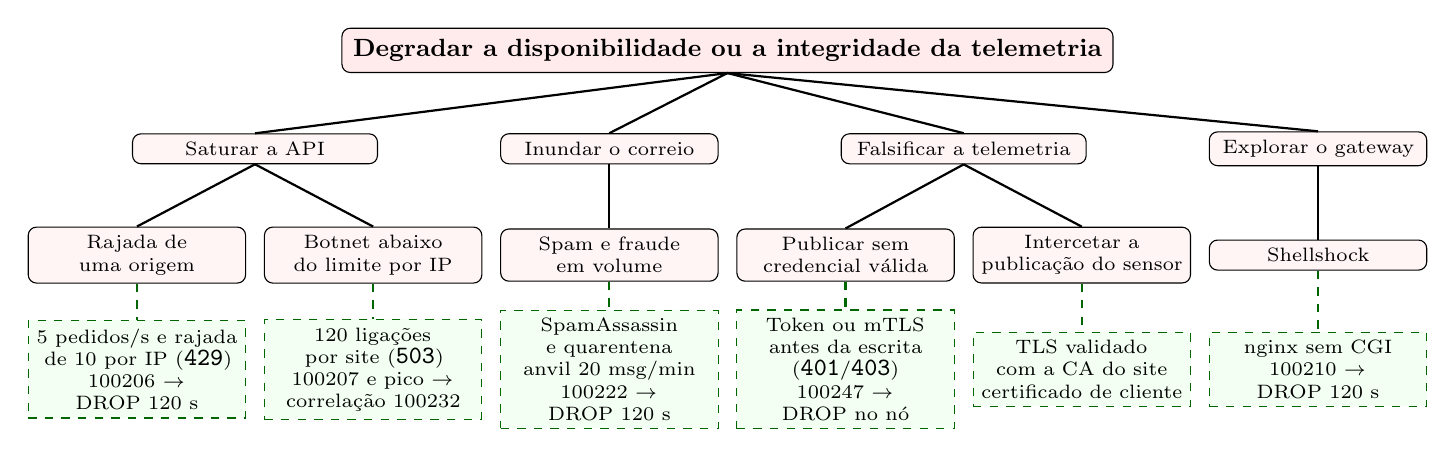
\begin{tikzpicture}[
  goal/.style={draw, rounded corners=3pt, align=center, font=\small\bfseries, fill=red!8, inner sep=4pt},
  atk/.style={draw, rounded corners=3pt, align=center, font=\scriptsize, fill=red!4, text width=2.55cm, inner sep=3pt},
  def/.style={draw=green!40!black, dashed, align=center, font=\scriptsize, fill=green!5, text width=2.55cm, inner sep=3pt},
  e/.style={thick}, d/.style={thick, green!40!black, dashed}
]
\node[goal] (g) at (0,0) {Degradar a disponibilidade ou a integridade da telemetria};
\node[atk,text width=2.9cm] (a1) at (-6,-1.25) {Saturar a API};
\node[atk] (a2) at (-1.5,-1.25) {Inundar o correio};
\node[atk,text width=2.9cm] (a3) at (3,-1.25) {Falsificar a telemetria};
\node[atk] (a4) at (7.5,-1.25) {Explorar o gateway};
\node[atk] (l1) at (-7.5,-2.6) {Rajada de uma origem};
\node[atk] (l2) at (-4.5,-2.6) {Botnet abaixo do limite por IP};
\node[atk] (l3) at (-1.5,-2.6) {Spam e fraude em volume};
\node[atk] (l4) at (1.5,-2.6) {Publicar sem credencial válida};
\node[atk] (l5) at (4.5,-2.6) {Intercetar a publicação do sensor};
\node[atk] (l6) at (7.5,-2.6) {Shellshock};
\node[def] (d1) at (-7.5,-4.05) {5 pedidos/s e rajada de 10 por IP (\code{429})\\100206 $\rightarrow$ DROP 120~s};
\node[def] (d2) at (-4.5,-4.05) {120 ligações por site (\code{503})\\100207 e pico $\rightarrow$ correlação 100232};
\node[def] (d3) at (-1.5,-4.05) {SpamAssassin e quarentena\\anvil 20 msg/min\\100222 $\rightarrow$ DROP 120~s};
\node[def] (d4) at (1.5,-4.05) {Token ou mTLS antes da escrita (\code{401}/\code{403})\\100247 $\rightarrow$ DROP no nó};
\node[def] (d5) at (4.5,-4.05) {TLS validado com a CA do site\\certificado de cliente};
\node[def] (d6) at (7.5,-4.05) {nginx sem CGI\\100210 $\rightarrow$ DROP 120~s};
\foreach \a in {a1,a2,a3,a4} \draw[e] (g.south) -- (\a.north);
\draw[e] (a1.south) -- (l1.north); \draw[e] (a1.south) -- (l2.north);
\draw[e] (a2.south) -- (l3.north);
\draw[e] (a3.south) -- (l4.north); \draw[e] (a3.south) -- (l5.north);
\draw[e] (a4.south) -- (l6.north);
\foreach \i in {1,...,6} \draw[d] (l\i.south) -- (d\i.north);
\end{tikzpicture}
\caption{Árvore de ataque e defesa. Os nós a vermelho são objetivos e ataques (alternativas). Os nós tracejados são as defesas aplicadas a cada folha, com a regra do Wazuh correspondente. Em qualquer folha, uma origem que volta a ser bloqueada passa a estar bloqueada em todos os serviços (100208).}
\label{fig:adtree}
\end{figure*}

\section{Cenários principais}
\subsection{Negação de serviço: rajada e botnet}
\emph{Ameaça e relevância.} Uma origem que envia pedidos a um ritmo elevado ocupa ligações do gateway e trabalho da análise e do armazenamento. Como o gateway é partilhado, a pressão sobre um site pode afetar o outro. Uma botnet distribui a carga para que cada origem fique abaixo do limite por IP.

\emph{Exploração.} No ensaio da rajada, \code{bot-1} envia 40 pedidos com concorrência~2, a carga do guião de DoS. No ensaio distribuído, os três bots fazem cerca de 10 pedidos/s cada durante 20~s. Na variante lenta, fazem cerca de 4 pedidos/s cada durante 40~s, abaixo do limite por IP. Em todos os casos, \code{client-user} consulta a API uma vez por segundo.

\emph{Prevenção e deteção.} O nginx admite 5 pedidos/s por IP e porta, com rajada de 10, e devolve \code{429} ao excesso. Também limita a 20 ligações por IP e a 120 por porta de site, com \code{503}. No Wazuh, cada \code{429} gera a regra~100204. Dez recusas da mesma origem em 10~s geram a 100206, que pede o bloqueio da origem durante 120~s na firewall do gateway, nas duas portas. Para o caso distribuído, a 100205 assinala 30 pedidos servidos à mesma origem em 10~s, e a 100207 dispara quando três origens diferentes atingem esse valor em 60~s. Esta última fica apenas como alerta, porque uma afluência legítima produz o mesmo sinal e a resposta ativa só bloquearia a última origem. No Prometheus global, \code{SharedGatewayRequestSurge} dispara quando os pedidos do último minuto excedem três vezes a média dos 30~minutos anteriores, com um mínimo de 120. O correlacionador junta a 100206 ou a 100207 com este pico ou com a latência do site e gera a regra~100232.

\emph{Resultado.} A rajada durou 14~ms: o nginx serviu 11 pedidos e recusou 29 com \code{429}. A regra~100206 disparou 1,5~s após o início e o bloqueio estava na firewall aos 1,6~s. A sonda de \code{bot-1} ficou sem resposta nas portas~80 e~8080 até à remoção da regra, 121~s depois. O cliente legítimo teve 167 respostas \code{200} em 167, com média de 2,3~ms. O pico global ficou em 115 pedidos por minuto, abaixo do limiar, como se pretende para uma rajada isolada.

No ensaio distribuído (Fig.~\ref{fig:ddos}), a 100207 disparou aos 5~s e os três bots foram bloqueados aos 7~s. Cada um recebeu 43 ou 44 respostas \code{200} e 14 \code{429}, e as tentativas seguintes ficaram sem resposta. O pico chegou ao Wazuh aos 37~s e o correlacionador gerou quatro eventos~100232, um para a botnet e um por origem bloqueada, todos no site Lisboa. Na variante lenta, os bots receberam 149 respostas \code{200} em 149 e nenhum foi bloqueado, porque a política admite esse ritmo. Ainda assim, a 100207 disparou aos 8~s e a correlação~100232 aos 47~s. Em ambos os ensaios, o cliente legítimo teve todas as respostas \code{200}, com um máximo de 3,8~ms. Nas cinco repetições da rajada e do DDoS (Tabela~\ref{tab:resultados}), a mediana do bloqueio foi de 1,6~s e de 6~s, respetivamente. A 100232 apareceu em quatro dos cinco DDoS. Na primeira repetição, o pico não passou o limiar: a média dos 30~minutos anteriores incluía o ensaio comparativo, com cerca de 3000 pedidos por minuto, e o limiar subiu. É o risco dos limiares adaptativos, aqui provocado pelos próprios ensaios.

\emph{Efeito no serviço.} As cargas anteriores são pequenas e não chegam a degradar o serviço. O ensaio \code{ataques/comparacao-protecao.sh} aplica a mesma carga duas vezes: três bots com dez clientes cada, durante 30~s, a pedir a lista de 1000 leituras, primeiro sem os limites do nginx e depois com a proteção normal (Tabela~\ref{tab:protecao}). Sem proteção, os bots receberam 2176 respostas \code{200}, cerca de 72 por segundo, e o tempo de resposta do cliente legítimo subiu de 2,4~ms para um p95 de 681~ms, porque a análise está limitada a 0,2~CPU por réplica. Com proteção, os bots receberam 56 respostas \code{200} e 1406 \code{429}, e a 100206 bloqueou os três entre 1,6 e 2,0~s após o início. O cliente legítimo manteve um p95 de 2,9~ms. O único pedido lento, com 339~ms, coincidiu com o primeiro segundo, em que a margem de rajada de cada bot ainda deixa passar onze pedidos. Sem proteção, o SIEM também detetou a botnet (100207) e correlacionou-a com o pico global (100232), mas nenhuma regra bloqueava, e o cliente legítimo esperou até 776~ms.

\begin{table}[!t]
\centering
\caption{Mesma carga sem e com proteção: 3 bots com 10 clientes cada, 30~s, \code{/api/temperatures?limit=1000}.}
\label{tab:protecao}
\setlength{\tabcolsep}{3pt}
\begin{tabular}{@{}>{\raggedright\arraybackslash}p{.20\columnwidth}>{\raggedright\arraybackslash}p{.33\columnwidth}>{\raggedright\arraybackslash}p{.40\columnwidth}@{}}
\toprule
Modo & Respostas aos bots & Legítimo: mediana / p95 / máx. \\
\midrule
Sem proteção & 2176 \code{200} & 2,4 / 681 / 776~ms; 60/60 \code{200} \\
Com proteção & 56 \code{200}, 1406 \code{429}; bloqueados aos 1,6--2,0~s & 2,3 / 2,9 / 339~ms; 68/68 \code{200} \\
\bottomrule
\end{tabular}
\end{table}

\begin{figure}[!t]
\centering
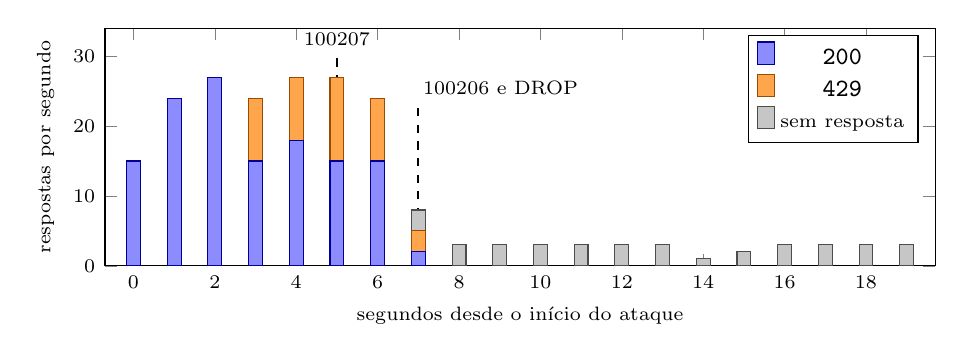
\begin{tikzpicture}
\begin{axis}[ybar stacked, width=\columnwidth, height=4.6cm, bar width=5pt,
  xlabel={segundos desde o início do ataque}, ylabel={respostas por segundo},
  xmin=-0.7, xmax=19.7, ymin=0, ymax=34, ytick={0,10,20,30},
  legend style={font=\scriptsize, at={(0.98,0.97)}, anchor=north east},
  tick label style={font=\scriptsize}, label style={font=\scriptsize}]
\addplot+[fill=blue!45, draw=blue!60!black] coordinates {(0,15) (1,24) (2,27) (3,15) (4,18) (5,15) (6,15) (7,2) (8,0) (9,0) (10,0) (11,0) (12,0) (13,0) (14,0) (15,0) (16,0) (17,0) (18,0) (19,0)};
\addplot+[fill=orange!70, draw=orange!60!black] coordinates {(0,0) (1,0) (2,0) (3,9) (4,9) (5,12) (6,9) (7,3) (8,0) (9,0) (10,0) (11,0) (12,0) (13,0) (14,0) (15,0) (16,0) (17,0) (18,0) (19,0)};
\addplot+[fill=gray!45, draw=gray!60!black] coordinates {(0,0) (1,0) (2,0) (3,0) (4,0) (5,0) (6,0) (7,3) (8,3) (9,3) (10,3) (11,3) (12,3) (13,3) (14,1) (15,2) (16,3) (17,3) (18,3) (19,3)};
\legend{\code{200}, \code{429}, sem resposta}
\draw[dashed, thick] (axis cs:5,0) -- (axis cs:5,30) node[above, font=\scriptsize] {100207};
\draw[dashed, thick] (axis cs:7,0) -- (axis cs:7,23) node[above right, font=\scriptsize, xshift=-2pt] {100206 e DROP};
\end{axis}
\end{tikzpicture}
\caption{Respostas recebidas pelos três bots no ensaio distribuído. O cliente legítimo, medido em paralelo, teve latências entre 2,0 e 3,8~ms.}
\label{fig:ddos}
\end{figure}

\begin{table*}[!t]
\centering
\caption{Ensaios com tráfego real a 21 de novembro de 2026. Na parte de cima, mediana e intervalo [mín.--máx.] de 5 repetições; na de baixo, ensaios únicos. Os instantes contam a partir do primeiro pedido do ataque. Nas repetições, o spammer desiste após 5 falhas seguidas.}
\label{tab:resultados}
\setlength{\tabcolsep}{4pt}
\begin{tabular}{@{}>{\raggedright\arraybackslash}p{2.3cm}>{\raggedright\arraybackslash}p{3.0cm}>{\raggedright\arraybackslash}p{4.8cm}>{\raggedright\arraybackslash}p{2.8cm}>{\raggedright\arraybackslash}p{4.1cm}@{}}
\toprule
Ensaio & Carga & Efeito no atacante & Cliente legítimo & Deteção e resposta \\
\midrule
Rajada HTTP & \code{bot-1}: 40 pedidos, concorrência 2 & 29 \code{429}; bloqueado nas portas 80 e 8080 aos 1,6 [0,4--2,2]~s, durante 121 [121--122]~s & 100\,\% \code{200}, máx. 4,0 [3,2--4,7]~ms & 100206 aos 1,0 [0,2--2,0]~s \\
DDoS distribuído & 3 bots, $\approx$10 pedidos/s, 20~s & 3 de 3 bloqueados, o último aos 6 [5--7]~s & 100\,\% \code{200}, máx. 2,7 [2,4--2,9]~ms & 100207 aos 4,8 [4,1--5,6]~s; 100232 em 4 de 5, aos 40 [35--47]~s \\
Spam e fraude & \code{bot-2}: até 40 mensagens, 0,1~s & 17 [13--20] aceites, 17 [13--20] em quarentena; bloqueio aos 2,3 [1,6--2,9]~s & 2 de 2 entregues; caixa com 2 novas & 100222 e DROP no correio \\
Shellshock & \code{bot-3}: 1 pedido & \code{404}; bloqueado aos 1,3 [0,7--1,9]~s & --- & 100210 aos 1,0 [0,2--1,5]~s \\
Publicação (extra) & \code{bot-3}: 7 pedidos HTTPS e 1 HTTP, Lisboa e Porto & 7 de 7 recusados, 0 leituras gravadas; bloqueado no nó K3s aos 1,5 [0,8--2,8]~s & --- & 100247 aos 1,1 [0,4--2,2]~s; 100245 aos 37 [33--43]~s \\
\midrule
\multicolumn{5}{@{}l}{\emph{Ensaios únicos}} \\
Botnet lenta & 3 bots, $\approx$4 pedidos/s, 40~s & 149/149 \code{200} cada; sem bloqueio & 79/79 \code{200}, máx. 3,1~ms & 100207 aos 8~s; 100232 aos 47~s \\
Publicação sem federação & idem, com a federação de Lisboa cortada & 7 de 7 recusados, 0 leituras gravadas & --- & 100231 do site inacessível; 100245 aos 78~s, não inibido \\
Reincidência & \code{bot-1}: 3 rajadas & 2.ª rajada: bloqueado 603~s no gateway, no correio e nos dois nós K3s & --- & 100208 1~s após a 2.ª rajada \\
Mesma carga sem e com proteção & 3 bots, 10 clientes cada, 30~s & ver Tabela~\ref{tab:protecao} & p95 de 681~ms sem proteção e 2,9~ms com & 100207 e 100232 nos dois modos; bloqueio só com proteção \\
Interceção & \code{bot-3} com certificado próprio & handshake recusado pelo sensor; com \code{-k}, token e leitura captados & --- & prevenção no cliente, sem alerta \\
\bottomrule
\end{tabular}
\end{table*}

\subsection{Spam e fraude}
\emph{Ameaça e relevância.} O servidor de correio de Lisboa é a entrada de mensagens para os utilizadores do site. Uma campanha em volume ocupa o filtro e enche a caixa. Uma mensagem de fraude pede dados bancários ou anuncia um prémio.

\emph{Exploração.} \code{bot-2} envia 40 mensagens com 0,1~s de intervalo, alternando um texto de farmácia com uma mensagem de lotaria que pede dados bancários. \code{client-user} envia uma mensagem legítima antes do ataque e outra durante o bloqueio.

\emph{Prevenção e deteção.} O Postfix entrega cada mensagem ao SpamAssassin através de um filtro, que regista o resultado, a pontuação e o IP de origem. Uma pontuação igual ou superior a 5 marca a mensagem. Três regras locais pontuam prémios, heranças e pedidos de credenciais com 4 pontos cada. A mensagem marcada volta ao Postfix e fica retida na fila \emph{hold} por uma regra \code{header\_checks}. O operador pode libertá-la ou apagá-la. A regra~100221 regista cada mensagem marcada. A~100222 dispara com cinco marcações da mesma origem em 60~s e bloqueia a origem na firewall de \code{lis-mail} durante 120~s. O anvil do Postfix limita cada cliente a 20 mensagens e 30 ligações por minuto.

\emph{Resultado.} O bloqueio entrou 1,1~s após a primeira mensagem. Onze mensagens foram aceites antes do bloqueio e as 29 seguintes esgotaram o tempo de ligação. As onze foram marcadas, com 6,2 pontos as de farmácia e 12,6 as de fraude, e ficaram todas em quarentena. A caixa só recebeu as duas mensagens legítimas, ambas com 0,0 pontos, incluindo a que foi enviada durante o bloqueio. O spammer voltou a ligar-se depois de a regra expirar. Nas cinco repetições, o bloqueio entrou aos 2,3~s de mediana, foram aceites entre 13 e 20 mensagens e todas ficaram em quarentena. No ensaio anterior às correções, 31 de 40 mensagens tinham chegado à caixa com 5,2 pontos. A margem de 0,2 pontos vinha da regra \code{ALL\_TRUSTED} ($-1{,}0$): sem \code{trusted\_networks}, o SpamAssassin considerava confiável qualquer relé da rede privada do laboratório. A configuração passou a confiar apenas no próprio servidor.

\subsection{Exploração do gateway: Shellshock}
\emph{Ameaça e relevância.} O CVE-2014-6271 permite executar comandos quando o Bash interpreta uma variável de ambiente que contém uma definição de função~\cite{cve}. Num servidor web, o vetor clássico é um CGI em Bash: o servidor copia cabeçalhos como o \emph{User-Agent} para variáveis de ambiente, e o comando que segue a função corre com os privilégios do servidor. O gateway é a única entrada da API e é partilhado pelos dois sites, por isso uma execução remota nele daria acesso aos dois. Mesmo sem vulnerabilidade, a tentativa identifica uma origem que procura serviços exploráveis, um comportamento típico de varrimentos automáticos e de botnets.

\emph{Exploração.} Como no guião do Wazuh, \code{bot-3} envia um pedido com a assinatura \code{() \{ :; \}; /bin/cat /etc/passwd} no \emph{User-Agent}, para um caminho CGI do gateway (\code{/cgi-bin/status}). Depois tenta voltar a ligar-se às duas portas a cada 5~s.

\emph{Prevenção e deteção.} A prevenção está na configuração. O nginx não executa CGI: só encaminha \code{/api/average} e \code{/api/temperatures} para a análise e devolve \code{404} a qualquer outro caminho. O Bash do gateway também está corrigido. A deteção usa o mesmo formato de log de acesso que o Apache das aulas. As regras~31166 e~31168 do Wazuh reconhecem a assinatura, com resposta de erro ou de sucesso, e a regra~100210 eleva-as ao nível~12 com resposta ativa: a origem fica bloqueada 120~s na firewall do gateway, nas duas portas. No guião, a mitigação acrescentava uma lista estática de IPs com má reputação. Essa regra (100100) continua configurada, mas com uma lista vazia, porque os IPs de ataque são os do próprio laboratório. A reincidência da Secção~\ref{sec:reputacao} calcula a reputação a partir do comportamento de cada origem.

\emph{Resultado.} O gateway respondeu \code{404} e nada foi executado. No primeiro ensaio, a 100210 disparou 0,5~s depois do pedido, o bloqueio estava ativo aos 0,7~s nas duas portas e foi retirado 121~s depois. Nas cinco repetições, a mediana foi de 1,0~s até à 100210 e de 1,3~s até ao bloqueio (Tabela~\ref{tab:resultados}). Tal como no guião, o servidor não é vulnerável e a defesa demonstrada é a deteção por assinatura seguida da contenção da origem. Uma variante da assinatura que escape às regras~31166 e~31168 passaria sem alerta.

\subsection{Reincidência e reputação partilhada}\label{sec:reputacao}
As respostas dos três cenários, e a da ingestão descrita na Secção~\ref{sec:publicacao}, bloqueiam a origem durante 120~s no serviço atacado. Uma origem que volta a atacar depois de o bloqueio expirar merece menos confiança, como num sistema de reputação. O correlacionador guarda, durante uma hora, os bloqueios de cada IP pelas regras~100206, 100210, 100222 e~100247. Os vários disparos da mesma rajada contam como um só incidente. Um novo bloqueio depois de o anterior expirar gera a regra~100208, e a origem fica bloqueada durante 10~minutos no gateway, no correio e nos dois nós K3s. À terceira vez, a regra~100209 alarga o bloqueio para uma hora. O historial é partilhado: um spammer que depois ataque a API já é tratado como reincidente. A lista branca do Wazuh exclui a bridge e os contentores de serviço, para que um teste ou um erro de configuração não isole a própria infraestrutura.

No ensaio \code{ataques/reincidente.sh}, \code{bot-1} repetiu a rajada HTTP três vezes. A primeira teve o bloqueio local de 122~s, só no gateway. A segunda começou 2~s depois de esse bloqueio expirar e gerou a 100208: a origem ficou bloqueada 603~s no gateway e também no correio e nos dois nós K3s, onde ainda não tinha atuado. Depois de limpar o historial, a terceira voltou aos 122~s.

O Wazuh tem uma opção nativa para reincidentes no agente (\code{repeated\_offenders}). No ensaio, o agente contou como reincidência o segundo disparo da 100206 na mesma rajada, à 20.ª recusa, e a primeira rajada ficou bloqueada 10~minutos. Por isso a contagem passou para o correlacionador, onde é feita por incidente e vale para todos os serviços.

\section{Implementações extra}
\subsection{Publicação não autorizada de leituras}\label{sec:publicacao}
\emph{Ameaça e relevância.} Uma leitura forjada entra nas médias e listas de um site e pode esconder uma avaria ou provocar uma decisão errada. É uma forma de sequestro de sinais, tema do programa que não teve guião prático: o atacante não precisa de derrubar o serviço, basta-lhe que o sistema aceite dados falsos.

\emph{Exploração.} A partir de \code{bot-3}, o atacante tenta gravar 99,9~°C no sensor de laboratório de Lisboa pelo NodePort~30441. Faz duas tentativas sem credencial e três com um token aleatório. Tenta também um identificador com \code{../}, um identificador inexistente e uma ligação por HTTP simples.

\emph{Prevenção e deteção.} A ingestão valida o formato do identificador e só aceita a credencial associada a esse ID. No token, compara o resumo SHA-256 em tempo constante. No mTLS, verifica a cadeia do certificado de cliente na CA de sensores do site e a sua impressão digital. A falta de credencial devolve \code{401}, a credencial recusada \code{403} e o identificador inválido \code{400}, sempre antes de contactar o armazenamento. A revogação atualiza o Secret partilhado pelas réplicas sem reiniciar o serviço. A ingestão escreve uma linha por recusa com o código, o identificador e o IP do cliente. O Service usa \code{externalTrafficPolicy: Local}, por isso o pod vê o IP real e não o do nó, e há uma réplica em cada nó. O agente Wazuh de cada nó lê o log do contentor. A regra~100246 regista cada recusa e a~100247 bloqueia durante 120~s, na firewall do nó, a origem com cinco recusas em 60~s. O bloqueio entra nas cadeias \code{INPUT} e \code{FORWARD}, antes das regras do Kubernetes, porque o tráfego de um NodePort é encaminhado para o pod. Em paralelo, o contador \code{ssle\_http\_auth\_rejections\_total} alimenta o alerta local \code{SsleIngestionAuthRejections} (três recusas em 5~min por site), que chega ao Wazuh como regra~100245 com o site e o serviço.

\emph{Resultado.} No ensaio das 17:41, as respostas foram duas \code{401}, quatro \code{403} e uma \code{400}, e a ligação por HTTP simples não teve resposta. Nenhuma leitura de 99,9~°C foi gravada. Cada recusa chegou ao Wazuh com o IP de \code{bot-3}. A 100247 disparou 2,4~s após o primeiro pedido e o \code{k3s-master} bloqueou a origem aos 3,1~s. As novas tentativas do atacante ficaram sem resposta até a regra expirar, 121~s depois. A 100245, que resume as recusas por site, chegou ao Wazuh cerca de um minuto depois, pelo Prometheus e pelo Alertmanager.

No primeiro ensaio do dia, esse alerta tinha ficado suprimido no Alertmanager. A causa era uma regra de inibição: quando o global perde a federação de um site, suprimia todos os avisos desse site, incluindo os de segurança. Um atacante que derrubasse o Prometheus de Lisboa conseguiria assim apagar o alerta de credenciais. Os alertas de segurança passaram a ter a etiqueta \code e a inibição deixou de os abranger. O ensaio de falha \code{tests/falha-federacao.sh} corta a federação de Lisboa e repete o ataque. \code{SiteMonitoringUnreachable} disparou 82~s depois do corte, o alerta de credenciais ficou ativo e não inibido, e a 100245 chegou aos 78~s. A federação recuperou 5~s depois de reposta.

\subsection{Interceção da publicação do sensor}
Este cenário aplica à ligação do sensor a parte de MitM do guião de DDoS. Um atacante que desvie o nome da ingestão para si, por DNS ou por rota, recebe a ligação do sensor. No ensaio, \code{bot-3} apresentou-se como \code{k3s-master.incus} com um certificado próprio. O desvio foi simulado no cliente com \code{curl --resolve} e \code{client-user} fez de sensor externo com a CA da ingestão de Lisboa. Com a ingestão verdadeira, o TLS foi aceite e a publicação sem credencial válida recebeu \code{401}. Com o nome desviado, o cliente recusou o certificado, o intercetor registou \emph{unknown CA} e não recebeu dados. Só com a validação desligada (\code{-k}) o intercetor captou o cabeçalho de autorização e a leitura e respondeu \code{202}, enganando o sensor. A proteção depende assim de cada sensor validar o servidor. Com mTLS, um token capturado também não basta, porque a chave privada do certificado de cliente nunca sai do sensor.

\section{Avaliação, recuperação e escalabilidade}
\subsection{Método e resultados}
Os ensaios correram a 21 de novembro na VM Kali, um de cada vez, com os scripts de \code{ataques/}. Cada script arranca os clientes necessários, regista o tráfego legítimo e as mudanças na firewall, recolhe os alertas do Wazuh e volta a parar os clientes no fim. O \code{ataques/repeticoes.sh} repetiu cinco vezes a rajada, o DDoS, o spam, a publicação (alternando Lisboa e Porto) e o Shellshock. Antes de cada ensaio, esperou que não houvesse bloqueios ativos e limpou o historial de reputação, para que as repetições fossem independentes. A Tabela~\ref{tab:resultados} apresenta a mediana e o intervalo. A evidência de cada ensaio está em \code{evidencias/}. Antes dos ensaios, a instalação passou o \code{check-after-boot.sh}, a aceitação \code{tests/k3s-defesas.sh}, os 25 testes unitários em Python (correlação, reputação, configuração dos sites e credenciais), os testes \code{promtool} das regras de alerta e o \code{wazuh-logtest} das regras novas. O mesmo conjunto, sem os ensaios na VM, corre no CI do repositório.

\subsection{Falhas encontradas pelos ensaios}
Até 20 de novembro, a rajada HTTP e o spam na topologia K3s tinham sido validados com registos sintéticos escritos diretamente no log do nginx e no journal do correio. Esse teste confirmava as regras e a resposta ativa, mas não o percurso do tráfego. Os ensaios com tráfego real revelaram três problemas que os registos sintéticos não mostravam: a inibição do alerta de credenciais, a correlação que procurava o nome de um alerta da topologia anterior e a confiança implícita do SpamAssassin na rede do laboratório. O correlacionador só reconhecia o alerta \code{GatewayRequestSurge} e etiquetas de site da instalação híbrida, por isso não produzia eventos~100232 desde 18 de novembro. Passou a aceitar o alerta da entrada partilhada, com \code{site=gateway}, para qualquer site servido pelo nginx. Cada correção foi verificada com o mesmo ensaio que a revelou.

\subsection{Gestão de falhas e escalabilidade}
A gestão de falhas segue o percurso de deteção, diagnóstico, isolamento e verificação da recuperação~\cite{m3400}. O ensaio \code{tests/falha-federacao.sh} percorre esse ciclo: corta a federação de Lisboa, o global deteta a perda com \code{SiteMonitoringUnreachable}, que chega ao Wazuh como regra~100231 com o site afetado, e a recuperação é confirmada depois de reposta a ligação. A deteção demorou 82~s e a recuperação 5~s. Num teste anterior, a ingestão de Lisboa passou de duas réplicas para uma, o sensor continuou a publicar e o Prometheus global observou os dois estados.

Na instalação atual, cada Prometheus local guarda 145 séries de 5 alvos. A federação envia ao global 13 séries agregadas por site, 1,7~kB por recolha em vez dos 39,9~kB do conjunto completo, cerca de 24 vezes menos. O número de séries locais cresce com as réplicas, enquanto o global mantém um indicador por serviço e por site. Um novo site exige uma entrada em \code{kubernetes/sites.json} com as suas portas. O gerador cria o namespace, os manifestos, o servidor nginx e o alvo da federação.

\subsection{Limitações}
Os dois sites partilham uma VM, um gateway e um cluster, o que concentra pontos únicos de falha. O armazenamento de cada site tem um único escritor SQLite. O bloqueio por IP pode atingir utilizadores atrás do mesmo NAT, e um bloqueio no gateway partilhado corta as consultas aos dois sites. A firewall atua sobre o tráfego posterior: os 40 pedidos da rajada foram todos tratados pelo nginx antes do bloqueio. Uma botnet abaixo do limite por IP é detetada mas não bloqueada. O limiar do pico aprende com a média recente, que um atacante paciente pode elevar aos poucos. Na ingestão, o bloqueio aplica-se no nó que recebeu as recusas; o outro nó só bloqueia depois de receber as suas. Um sensor com credencial válida que inunde a ingestão não é limitado. Um certificado de cliente recusado durante o TLS fica fora do contador e do registo. A política \code{Local} exige uma réplica de ingestão em cada nó. O spam marcado fica em quarentena, mas a classificação admite falsos negativos e a quarentena exige decisão do operador. O historial de reputação vive na memória do correlacionador e perde-se se este reiniciar. O p95 que cada serviço exporta mede o tempo dentro do serviço e não a espera em fila: no ensaio sem proteção ficou abaixo de 0,1~s, enquanto o cliente esperava até 776~ms. As cargas são pequenas e tudo corre numa só máquina, por isso os tempos indicam a ordem de grandeza e não a capacidade sustentada do sistema.

\section{Conclusões}
Cada entrada do sistema tem o controlo no ponto em que o pedido chega. O nginx limita o trabalho admitido e não executa CGI, o correio classifica e retém o spam, e a ingestão só grava leituras autorizadas. O Wazuh acrescenta a resposta por origem nos quatro pontos de entrada, a reputação partilhada entre serviços e a correlação com os sintomas que o Prometheus observa. A comparação com a mesma carga mostra o que a deteção sozinha não faz: sem os limites do nginx, o SIEM detetou a botnet e correlacionou-a com o pico, mas o cliente legítimo esperou até 776~ms. Com os limites, os bots ficaram bloqueados em 2~s e o cliente manteve 2,9~ms de p95. Nas cinco repetições, o atacante perdeu o acesso com uma mediana entre 1,3 e 2,3~s nos ataques de uma origem e de 6~s no ataque distribuído, e o cliente legítimo não teve erros. A correlação 100232 apareceu em quatro dos cinco DDoS. Na repetição sem correlação, a referência do limiar adaptativo ainda incluía o ensaio comparativo, que tinha elevado o volume considerado normal. Os ensaios com tráfego real foram também o método mais útil para encontrar falhas que os testes sintéticos não mostravam.

O trabalho futuro passa por limitar a taxa de publicação por sensor autenticado, propagar o bloqueio da ingestão aos dois nós, guardar a reputação de forma persistente, medir a latência no nginx em vez de dentro de cada serviço e separar os sites em máquinas distintas. O Projeto~2 pode partir daqui com a tolerância a falhas do armazenamento e a rotação das credenciais dos sensores.

\section*{Declaração de uso de IA}
Foram usados Claude Code e Codex no apoio à implementação, à execução e revisão dos ensaios e à redação do artigo. O autor validou as alterações na VM e cruzou cada resultado apresentado com os registos de execução em \code{evidencias/}.

\begin{thebibliography}{99}
\bibitem{course} V. Cunha e S. Vaz, ``Projeto 1 e guiões práticos'', Segurança em Sistemas de Larga Escala, Universidade de Aveiro, 2026.
\bibitem{knet} Kubernetes, ``Network Policies'', documentação. \url{https://kubernetes.io/docs/concepts/services-networking/network-policies/}
\bibitem{prom} Prometheus, ``Federation'', documentação. \url{https://prometheus.io/docs/prometheus/latest/federation/}
\bibitem{wazuh} Wazuh, ``Rules syntax'', documentação. \url{https://documentation.wazuh.com/current/user-manual/ruleset/ruleset-xml-syntax/rules.html}
\bibitem{wazuhar} Wazuh, ``Active Response'', documentação. \url{https://documentation.wazuh.com/current/user-manual/capabilities/active-response/index.html}
\bibitem{bhatt} S. Bhatt, P. K. Manadhata e L. Zomlot, ``The Operational Role of Security Information and Event Management Systems'', \emph{IEEE Security \& Privacy}, vol. 12, n.º 5, pp. 35--41, 2014.
\bibitem{m3400} ITU-T, ``M.3400: TMN management functions'', recomendação, 2000.
\bibitem{mirkovic} J. Mirkovic e P. Reiher, ``A Taxonomy of DDoS Attack and DDoS Defense Mechanisms'', \emph{ACM SIGCOMM Computer Communication Review}, vol. 34, n.º 2, pp. 39--53, 2004.
\bibitem{jung} J. Jung, B. Krishnamurthy e M. Rabinovich, ``Flash Crowds and Denial of Service Attacks: Characterization and Implications for CDNs and Web Sites'', em \emph{Proc. WWW}, 2002, pp. 293--304.
\bibitem{adtree} B. Kordy, S. Mauw, S. Radomirović e P. Schweitzer, ``Foundations of Attack--Defense Trees'', em \emph{Formal Aspects of Security and Trust}, Springer, 2010.
\bibitem{nginx} nginx, ``Module ngx\_http\_limit\_req\_module'' e ``Module ngx\_http\_limit\_conn\_module'', documentação. \url{https://nginx.org/en/docs/}
\bibitem{apachempm} Apache HTTP Server, ``Multi-Processing Modules (MPMs)'' e ``mod\_ratelimit'', documentação da versão 2.4. \url{https://httpd.apache.org/docs/2.4/mpm.html}
\bibitem{sa} Apache SpamAssassin, ``Mail::SpamAssassin::Conf'', documentação (\code{trusted\_networks}). \url{https://spamassassin.apache.org/}
\bibitem{cve} NIST, ``CVE-2014-6271'', National Vulnerability Database. \url{https://nvd.nist.gov/vuln/detail/CVE-2014-6271}
\end{thebibliography}
\end{document}
